% Harmadik és negyedik előadás

\chapter{Disszipációkezelés}

\section{A disszipációkezelés fontossága}
A processzorok fejlesztésének két iránya van: teljesítmény növelése és a fogyasztás csökkentése.
A fejlesztés fókusza folyamatosan a disszipáció csökkentése felé tolódott, mivel rájöttek, hogy a teljesítmény fő korlátja a disszipáció.

\section{A disszipáció}
A disszipáció két komponensből áll: dinamikus (működés közbeni) és statikus.
A tápegység szempontjából a processzor egy szórt kapacitás, amit a felfutó órajelen fel kell tölteni, a lefutón pedig egy ellenálláson keresztül le kell vezetni.
A töltés-kisülés fogyasztása a dinamikus disszipáció.
A statikus disszipáció a lezárt tranzisztorok szivárgási áramából adódik.
A teljes disszipáció a kettő összege.

\subsection{Kiszámítása}
A dinamikus disszipáció kiszámításához a processzor aktív tranzisztorait egy áramkörrel modellezhetjük (\ref{fig:dyndis}).
\begin{figure}[H]
    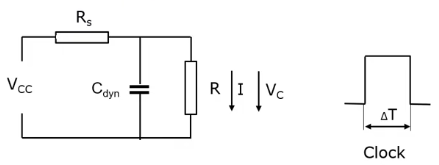
\includegraphics[width=0.8\textwidth]{dyndis}
    \centering
    \caption{Aktív tranzisztorok modellje}
    \label{fig:dyndis}
\end{figure}
Ebből a dinamikus disszipáció kiszámítása:
\begin{equation}
    D_d=2*C_dyn*V_{cc}^2*f_c
\end{equation}
Az órafrekvenciával lineáris, mivel a töltés-kisülések mennyisége függ tőle.

\section{TDP}
Thermal Design Power, azaz tervezési hőérték.
Egy számításigényes alkalmazás futtatása közbeni maximális disszipációt jelenti.
Fontos, hogy nem teljesen pontos érték.
Az OEM-ek ez alapján tervezik a hűtés rendszereket, aminek legalább ezt a TDP értéket el kell vezetnie úgy, hogy a tranzisztorok hőmérséklete nem megy kb. 80-90°C fölé.
A kategóriák jellemző TDP értékeit mutatja a \ref{fig:tdp}. ábra.
\begin{figure}[H]
    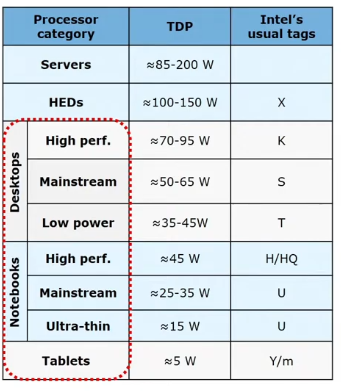
\includegraphics[width=0.6\textwidth]{tdp}
    \centering
    \caption{Processzor osztályok jellemző disszipációja}
    \label{fig:tdp}
\end{figure}
A TDP korlátozza az alapfrekvenciát.
A Turbo működéséhez jóval több watt szükséges.

\section{Intel processzorok disszipációja a fejlődés során}
A \ref{fig:evointel}. ábrán az Intel processzorok lapkamérethez viszonyított disszipációjának növekedése látható az órajel növekedésével.
\begin{figure}[H]
    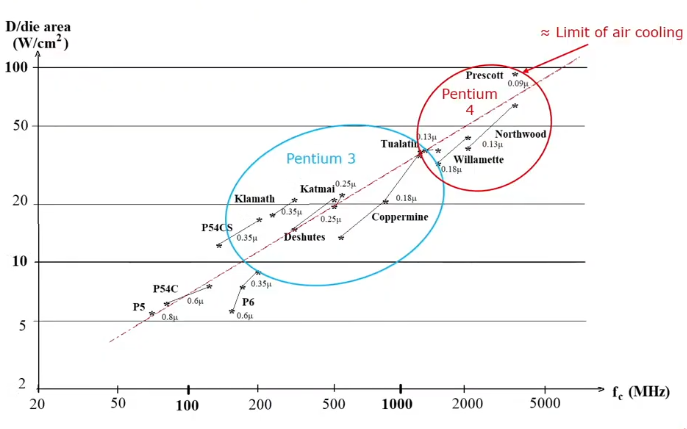
\includegraphics[width=0.8\textwidth]{evointel}
    \centering
    \caption{Disszipáció változása az órajel függvényében}
    \label{fig:evointel}
\end{figure}
Látható, hogy a Pentium 4 Prescott mag már közel 100 wattot adott le cm\textsuperscript{2}-enként, ami a léghűtés fizikai határa.
Az Intel 2000-ben azt várta a Pentium 4 családtól, hogy 10 évig gyártásban marad és 10 GHz órajelet fog elérni.
Ehelyett 2004-ben 4 GHz-nél megakadt a fejlesztés.
A Prescott család bizonyos tagjait kénytelenek voltak visszavonni túlmelegedési problémák miatt.

Ezzel az Intel 2003-tól a nyers teljesítményről áthelyezte a hangsúlyt a teljesítmény per watt, azaz a hatékonyság növelésére.
Összefoglalva a tervezési paradigmák változását mutatja a \ref{fig:paradigm}. ábra.
\begin{figure}[H]
    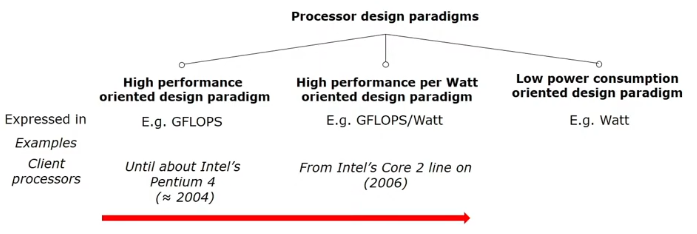
\includegraphics[width=0.8\textwidth]{paradigm}
    \centering
    \caption{Processzor tervezési paradigmák}
    \label{fig:paradigm}
\end{figure}

\section{Disszipációcsökkentő kezdeményezések}
A disszipáció kezelésére megszületett az Energy Star kezdeményezés, az AMD pedig célul tűzte ki, hogy 2014 és 2020 között 20x-osára emeli a hatékonyságot.

\subsection{Energy Star}
Az amerikai környezetvédelmi hatóság indította 1992-ben, az energiatudatosság elterjesztésére a processzoroknál.
Több verziója volt, a legfontosabb az 5., amit 2009-ben adtak ki, a Pentium 4 problémái után.
Lényege, hogy a processzorokra kiszámítják az éves inaktív állapotú energiafogyasztást, és ha egy modell a határérték alatt van, akkor használhatja az Energy Star jelölést.
A különböző inaktív állapotok súlyozása kategóriánként eltér.

\subsection{Az AMD hatékonysági kezdeményezése}
2014-ben jelentették be, hogy növelni szeretnék a teljesítmény per watt arányt.
2009-től 2014-ig 10x-es hatékonyság növekedést értek el, ehhez képest szerettek volna további 25x-ös javulást 2020-ra.
2020-ban bejelentették, hogy a Zen 2 alapú Ryzen processzoraikkal elérték a célt, 32x-es növekedéssel.

\subsection{Szerverek energiahatékonysága}
A szervereknél kiemelten fontos a hatékonyság, mivel egy adatközpont több MW áramot is fogyaszthat.
A szuperszámítógépeket hatékonyság szerint is rangsorolják, erre szolgál a Green500-as lista.

\section{ACPI}
Az inaktív állapot definiálása az Energy Star-hoz az ACPI (Advanced Configuration and Power Interface) szabvány segítségével lehetséges.
Ez egy nyílt szabvány, ami definiálja a számítógép állapotait.
Az állapotot globális (Gi), teljesítmény (Pi), inaktív (Ci) és alvó (G3) állapotok jellemzik (\ref{fig:acpi}. ábra).
\begin{figure}[H]
    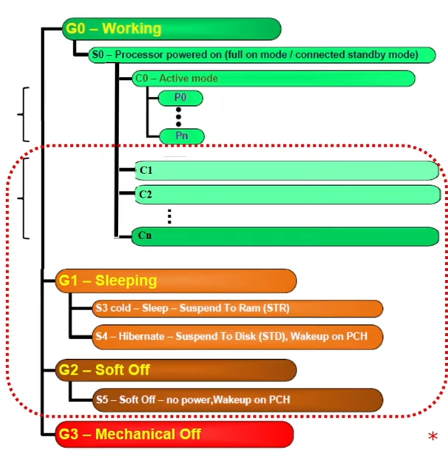
\includegraphics[width=0.5\textwidth]{acpi}
    \centering
    \caption{ACPI állapotok}
    \label{fig:acpi}
\end{figure}

Globális állapotok:
\begin{itemize}
    \item G1: OS által kezdeményezett leállás, kontextus mentéssel
    \item G2: OS által kezdeményezett leállás, kontextus mentés nélkül, tápellátás megmarad
    \item G3: mechanikai kikapcsolás
\end{itemize}

\section{A disszipációkezelés technikái}
A disszipáció kezelése sokféleképpen történhet, a tranzisztorok tervezésétől az áramkörökön és a processzoron át egészen a platform és operációs rendszer szintekig.

\subsection{Kezelés áramköri szinten}
Két jelentős technológia:
\begin{itemize}
    \item óra kapuzás
    \item tápfeszültség kapuzás
\end{itemize}

\subsubsection{Óra kapuzás}
Az éppen inaktív áramkörök elé egy AND kapu kerül, ami inaktivitás esetén nem küld órajelet az áramkörre, így csökkentve a fogyasztást.
A statikus disszipáció viszont továbbra is fennmarad.
Implementációja történhet finom vagy durva szemcsézettséggel.
A finomnál kis áramköri egységeket külön-külön kapuznak, míg a durva szemcsézés több modult kapuz egyszerre.
Az óra kapuzást korán, már 1996-ban is alkalmazta a DEC cég az Alpha processzoraiban (lebegőpontos egységeket kapuzták).
Mivel a technológia jól bevált, hamar elterjedt, az Intel a Pentium 4-től használja, ma már teljesen általános.

\subsubsection{Tápellátás kapuzása}
Az óra kapuzás továbbfejlesztése, nagyobb áramköri egységekre használják mint pl. mag vagy memória kontroller.
Az egység inaktivitása esetén a komplett tápellátást lekapcsolja az egységről, így a dinamikus és a statikus disszipációt is megszüntetve.
A többmagos processzorokban a processzormagok külön-külön kapuzhatók.

A tápfeszültség kapuzás előfeltétele a Turbo Boost technológiának, mivel a Turbo órajel a processzor fogyasztása és a TDP közötti hőtartalékot felhasználva emeli meg az órajelet.
Ehhez elegendő hőtartalékot kell biztosítani, amit nagyban elősegít a kapuzás.

A tápellátás kapuzást az Intel vezette be a Nehalem processzorokkal 2008-ban.
Később az AMD és az IBM is átvette.

Implementáció szerint először (Nehalem) csak a magokat kapuzták, később több egységre is kiterjedt mint pl. L3 cache, GPU, memória kontroller.
Az Intel a Westmere, Sandy Bridge és Ivy Bridge folyamatosan terjesztette ki a kapuzást, az AMD a Bulldozer családdal gyakorlatilag minden alapegységet kapuzott.

A tápellátás megszüntetése történhet a pozitív pólus vagy a föld elvágásával is.

\subsubsection{Integrált tápegységek - Intel FIVR}
Az Intel a Haswell családdal továbbfejlesztette az energiaellátást, a tápegység (voltage regulator) bizonyos részeinek processzorlapkára helyezésével.
Ez a FIVR (Fully Integrated Voltage Regulator), ami eltérő feszültséggel tudja ellátni a processzor különböző részeit, így a kapuzás fölöslegessé vált.

Ezt a technológiát a Haswell és Broadwell processzorok után felfüggesztették, mivel az integrált tápegység a processzor disszipációjához adott hozzá, így csökkentve az elérhető órajelet.
A Skylake-el kezdődően tehát ideiglenesen visszatértek a teljesítmény kapuzásra.

\subsubsection{Feszültség lekapcsolás előkészítése}
Mielőtt egy magról lekapcsolnánk a tápot, a gyorsítótárat vissza kell írni a következő szintű gyorsítótárba, vagy ha az nem elérhető, memóriába.
A processzor végrehajtási állapotát (kontextus, azaz a regiszterek állapota) is el kell menteni egy következő szintű cache-be, vagy a memóriába, esetleg SRAM-ba.
A táp lekapcsolással együtt a magról lekapcsolják az órajelet és az órajel generátort is.

\subsubsection{A kontextus mentése}
A kontextus mentése történhet:
\begin{itemize}
    \item memóriába (AMD használta pl. Bulldozer, Piledriver, Excavator, Bobcat, Jaguar)
    \item következő szintű gyorsítótárba (AMD Jaguar, Puma)
    \item magonkénti SRAM-ba (Intel processzorok)
\end{itemize}

\subsection{Kezelés platform szinten}
Platform szinten bonyolult a disszipáció kezelés, mivel részt vesz benne a processzor, az IO eszközök, a BIOS és az OS is.
Az első ilyen megoldások az Inteltől származnak (SL), később a Microsofttal összefogva fejlesztettek (APM, nem terjedt el).
Később több gyártó is bekapcsolódott, így alakult ki a nyitott ACPI szabvány (1996-tól máig használják).

\subsubsection{Az ACPI fejlődése}
Az ACPI 1.0 verziót a Windows 95, 98, 2000 és NT 4.0 rendszerek támogatták.
Az XP és a Server 2003 rendszerek már az ACPI 2.0-t használták, amiben már jelen volt a DVFS (Dynamic Voltage and Frequency Scaling) és nagyban elősegítette a disszipáció kezelését.
A többmagos és többszálas rendszerek támogatása az ACPI 3.0-ban jelent meg, ezt a Vista, 7 és Server 2008 operációs rendszerek használták.
A 4.0 kevésbé jelentős, de az 5.0 egy új szemléletet vezetett be: Collaborative Processor Performance Control, aminek során az operációs rendszer csak átadja a processzornak, hogy a felhasználó a teljesítményt vagy az alacsony fogyasztást preferálja, majd ezután a többi döntést a processzor hozza meg hardveresen.
A fejlődés folytatódott, de a 6-os verziónak nem voltak jelentős újításai.

\subsection{Kezelés CPU szinten}
Kétféle kezelési lehetőség:
\begin{itemize}
    \item aktív magok kezelési technikái:
    \begin{itemize}
        \item energiafogyasztás csökkentése:
        \begin{itemize}
            \item DVFS - dinamikus feszültség és frekvencia kezelés
            \item CPPC
            \item AVFS - adaptív feszültség és frekvencia kezelése
        \end{itemize}
        \item Turbo Boost: a TDP hőtartalékát felhasználva megemeli a processzor az alap frekvenciáját ideiglenesen
    \end{itemize}
    \item inaktív magok kezelési technikái (ACPI alapú, C állapoton keresztül): a kihasználatlan magot egyre mélyebb alvó állapotba helyezi a rendszer.
\end{itemize}

\subsubsection{DVFS - Dynamic Voltage and Frequency Scaling}
\paragraph{Egymagos rendszerek}\mbox{}\\
A DVFS (egymagos, egyszálas processzoroknál) alapelvei:
\begin{itemize}
    \item a dinamikus fogyasztás kiszámítása:
        \begin{equation*}
            D_d = const * V_{cc}^2 * f_c
        \end{equation*}
    \item a szükséges magfeszültség ($V_{cc}$) ahhoz, hogy stabil órajelet lehessen generálni közel egyenesen arányos az órafrekvenciával
        \begin{equation*}
            V_cc = const * f_c
        \end{equation*}
    \item tehát a dinamikus disszipáció közel köbösen aránylik a frekvenciához:
        \begin{equation*}
            D_d = const * f_c^3
        \end{equation*}
\end{itemize}
Következmény, hogy a disszipáció csökkentésére nagyon hatékony eszköz a frekvencia csökkentése.
Fontos, hogy a frekvencia csak addig csökkenthető, amíg ez nem rontja a felhasználói élményt.

A DVFS a P (performance) állapotokon alapul, amiket az ACPI 2. verziója tartalmazott.
A P állapotok munkapontok, amik a magfrekvencia és órafrekvencia kettősöket adják meg (\ref{fig:p}. ábra).
\begin{figure}[H]
    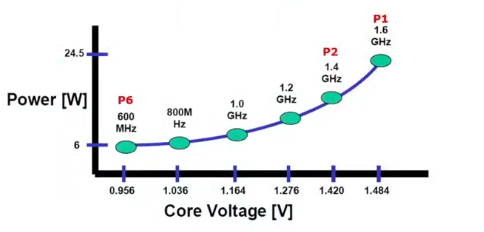
\includegraphics[width=0.8\textwidth]{p}
    \centering
    \caption{Az Intel Pentium M processzor munkapontjai}
    \label{fig:p}
\end{figure}
Látható, hogy a legalacsonyabb állapotban csak 6 watt a disszipáció, a legmagasabbban pedig már 24.5 watt.
A cél tehát a lehető legalacsonyabb fogyasztású P állapotban tartani a processzort, ha ez megtehető a felhasználói élmény rontása nélkül.
A legmagasabb teljesítményű és fogyasztású állapot a P1.

Itt nagyon fontos szerepet kap az OS, mivel neki kell eldöntenie, hogy melyik az a P állapot, ami még nem rontja érezhetően a teljesítményt.
Ehhez az OS vizsgálja a CPU kihasználtságot: megnézi, hogy egy adott időablakot az ütemező hány százalékban használ ki.
Pl.: ha a CPU mag 2 GHz-en működik, de a kihasználtság csak 50\%, akkor minden második óraciklus elvesztegetett.
Ezért a frekvencia levihető 1 GHz-re, érezhető lassulás nélkül.
Ez alapján az OS kiválasztja a P állapotok közül az optimális munkapontot.
Ha megtörtént a kiválasztás, az OS a CPU-val egy regiszter interfészen keresztül közli a döntést.
Ezt az interfészt az ACPI standard határozza meg.
Ezután ezt a regisztert lekérdezi a PCU (Power Control Unit) és beállítja a frekvenciát.
Ez a rendszer igényvezérelt skálázást tesz lehetővé.

\paragraph{Többmagos rendszerek}\mbox{}\\
Többmagos rendszereknél az OS a taskokat szálakhoz, és nem magokhoz rendeli.
Ezért a kihasználtságot is szálakra vizsgálja.
A DVFS lépései több mag és több szál esetén:
\begin{itemize}
    \item szál kihasználtság meghatározása
    \item kihasználtság alapján legjobb P állapot kiválasztása
    \item ha több szál van egy magon, koordinálni kell a kiválasztott P állapotokat (egy mag csak egy feszültségen működhet)
    \item az igényelt P állapot kommunikálása a processzorral
    \item a PCU beállítja az igényelt magfeszültséget és órajelet
\end{itemize}

\paragraph{Szál kihasználtság meghatározása}\mbox{}\\
Először azt figyelték, hogy az idő hány százalékában nincs ütemezendő szál, viszont ez körülményes volt.
Ezért 2006-tól az Intel bevezetett szálanként két gépi 64 bites regisztert, amiket számlálóként használ.
A számlálókat csak akkor lépteti a processzor, ha az adott szálhoz tartozó logikai processzor aktív (C0) állapotban van.
Az egyik számlálót az alapfrekvencia ütemében inkrementálják, a másikat pedig a pillanatnyi órajel ütemében.
A kettő aránya megadja a processzor kihasználtságát.

\paragraph{P állapot meghatározása}\mbox{}\\
A kihasználtság alapján meghatározható a legmegfelelőbb P állapot (\ref{fig:p2}. ábra).
\begin{figure}[H]
    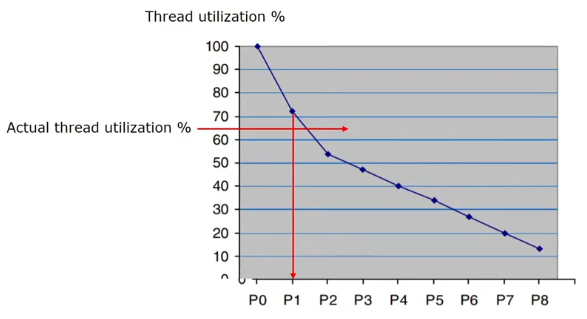
\includegraphics[width=0.7\textwidth]{p2}
    \centering
    \caption{P állapot meghatározása}
    \label{fig:p2}
\end{figure}

\paragraph{Több szál koordinálása egy magon}\mbox{}\\
Ha egy mag több szálat futtat, mindig a teljesítmény igényesebb szálhoz kell igazítani a mag állapotát.
Ha több mag van egy közös órajelről táplálva, szintén a legnagyobb teljesítmény igényű szálat futtató maghoz kell igazodni.
Az újabb rendszerek már képesek magonként különböző P állapotokat kezelni, így a magok közötti koordináció nem szükséges.

\paragraph{Kiválasztott P állapot kommunikációja}\mbox{}\\
Erre a performance control (IA32\_PERF\_CTL) belső regiszterek szolgálnak, amibe az OS írhat.
A regiszterben az alsó kettő byte szolgál a feszültség és a frekvencia megadására.
A frekvencia megadása szorzófaktorral történik, pl. 133 MHz busz frekvenciánál 34-es szorzó 34x133 MHz-t jelent.
Ennek a regiszternek a kódolása nem publikus.

\paragraph{PCU működése}\mbox{}\\
A performance control regiszter kiolvasása után a PCU beállítja a szükséges paramétereket.

\paragraph{DVFS az Intel Nehalem processzorokon}\mbox{}\\
A Nehalem mikroarchitektúrára épülő CPU-knál vezették be először a PCU használatát.
Működése a \ref{fig:pcu}. ábrán látható.
\begin{figure}[H]
    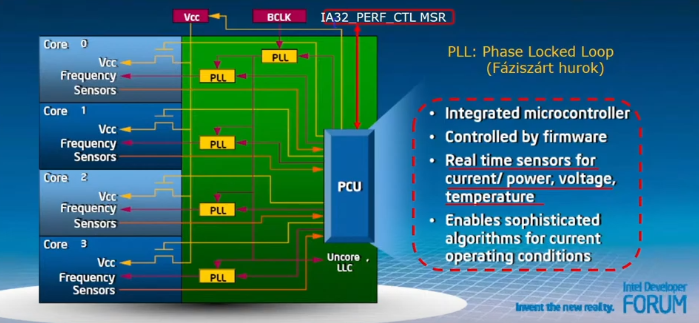
\includegraphics[width=0.8\textwidth]{pcu}
    \centering
    \caption{PCU az Intel Nehalem processzorokban}
    \label{fig:pcu}
\end{figure}

\subsubsection{A DVFS továbbfejlesztése}
A DVFS-nek két továbbfejlesztett változata van:
\begin{itemize}
    \item CPPC: az OS csak iránymutatással látja el a PCU-t, a precíz feszültség és órajel szabályzást a PCU végzi.
    \item AVFS: a DVFS biztonsági zónáját csökkenti, a teljesítmény növelése vagy a disszipáció csökkentése érdekében.
\end{itemize}
A CPPC-t az Intel a 2015-ös Skylake óta használja (SpeedShift), az AMD pedig a 2019-es Zen 2 alapú Ryzen 3000 óta.
Az AVFS egy régebbi rendszer, az IBM 2007 óta használja, a Samsung 2015-től (Galaxy S6), az AMD pedig a régebbi processzoraiban.

\subsubsection{CPPC - Collaborative Processor Performace Control}
A CPPC-t az ACPI 5.0 szabvány definiálja, az ACPI 2.0 alapú DVFS-t váltja le ez a technológia.
Ehhez szintén szükséges OS támogatás, ami a Windows 10 2015 őszi frissítésével jelent meg.

A DVFS-nél az OS nézi a kihasználtságot és küldi el a szükséges P állapot paramétereket.
Hátránya, hogy a kihasználtság vizsgálata nagy időablakban történik, így a rendszer lassú, csak ritkán tudja módosítani a P állapotokat.
A gyorsításához a lehető legjobban ki kell küszöbölni az OS-t, erre szolgál a CPPT.
Ez a gyorsulás látszik a \ref{fig:cppc}. ábrán.
\begin{figure}[H]
    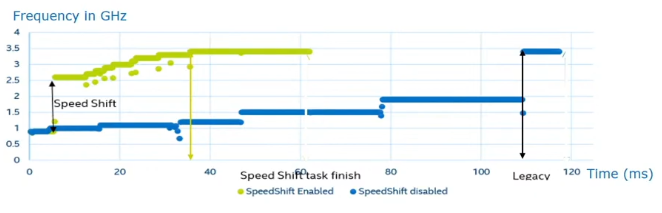
\includegraphics[width=0.8\textwidth]{cppc}
    \centering
    \caption{Intel SpeedShift (CPPC) és DVFS frekvencia átállási ideje}
    \label{fig:cppc}
\end{figure}

A CPPC-nél az OS csak felhasználói igényeket továbbít, mint pl. a teljesítmény vagy a fogyasztás preferálása.
Ezután a vezérlést átadja a PCU-nak, ami önállóan beállítja a szükséges paramétereket, valamint végrehajt optimalizációkat is.
Az optimalizálásokat több algoritmus segítségével hajtja végre.
Az operációs rendszer felügyeli a PCU működését és hiba esetén beavatkozhat.

További fejlesztés még a DVFS-hez képest, hogy a diszkrét munkapontok helyett bármilyen szorzó beállítható.
Ezzel finomabb szabályozás valósítható meg.

Az alacsonyabb felfutási időnek köszönhetően a CPPC segítségével nagyobb teljesítmény érhető el (\ref{fig:pcmark}. ábra).
\begin{figure}[H]
    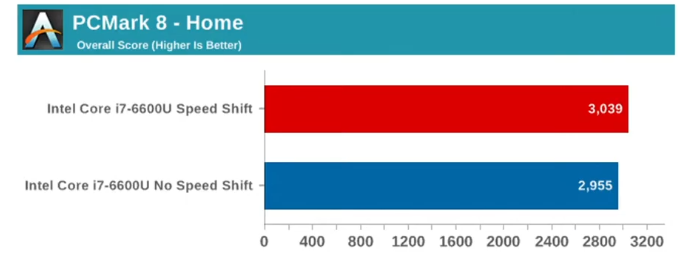
\includegraphics[width=0.8\textwidth]{pcmark}
    \centering
    \caption{Benchmark eredmények CPPC-vel és anélkül}
    \label{fig:pcmakr}
\end{figure}
A teljesítmény javulása viszont nem számottevő (kb 1.5\%).
Más alkalmazásoknál kb. 20\% javulás érhető el.
A további gyorsításért az Intel a Kaby Lake processzorokban javított a SpeedShift technológián, a korábbi 35 ms-os felfutási időt 10 ms-re csökkentették.

Az AMD CPPC Implementációja már egy korszerűsített CPPC változatot valósít meg, ami az ACPI 5.1 szabványból származik.
A felfutási időt az AMD 1 ms környékére csökkentette.

\subsubsection{AVFS}
A DVFS-nél az OS előre meghatározott frekvencia-feszültség párosokból választ működési pontokat.
Ezeket a működési pontokat minden CPU fejlesztése során mérésekkel határozzák meg (adott frekvenciához melyik az a legkisebb feszültség, amin még stabilan működik a CPU), majd ezt egy biztonsági értékkel növelik (guard band), hogy rosszabb körülmények is jó legyen a CPU.
Ilyen körülméyek pl.:
\begin{itemize}
    \item gyártási eljárás miatti eltérések
    \item processzor belsejében tápfeszültségek eltérései
    \item processzor hőmérséklete
    \item processzor öregedése
\end{itemize}
A gyártási eljárás figyelembe vételénél azokkal a legyártott darabokkal kell számolni, amiknek a legmagasabb a minimum magfeszültsége.
Probléma, hogy mindezek miatt a biztonsági sávot nagyon nagynak kell megválasztani.

Az AVFS erre jelent megoldást, csökkenti a szükséges biztonsági sávot.
Alapja, hogy nem a legrosszabb esetet veszzük figyelembe, hanem helyben történik a minimális feszültség meghatározása.
A helyi mérés kritikus út monitorokkal valósul meg, tehát a kritikus áramköri részeken áthaladó jeleket méri a processzor és hasonlítja össze az órajellel.
Ha a jel hamarabb érkezik meg, mint a következő órajel, akkor még növelhető a frekvencia vagy csökkenthető a feszültség.
Ha pont egyszerre, akkor elérte a jó beállítást.
Ha pedig később érkezik meg a vizsgált jel, mint az órajel, akkor csökkenteni kell a frekvenciát, vagy növelni a feszültséget.
Ezeket az eseteket mutatja a \ref{fig:avfs}. ábra.
\begin{figure}[H]
    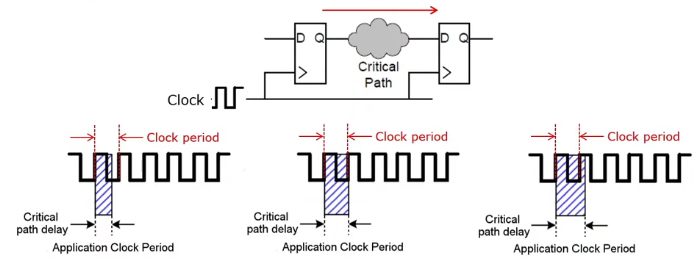
\includegraphics[width=0.8\textwidth]{avfs}
    \centering
    \caption{Órajel és frekvencia beállítása kritikus út monitorozással}
    \label{fig:avfs}
\end{figure}
Az AVFS a kritikus út monitorok jelzései alapján be tud állítani egy, a gyártásnál meghatározottnál jóval kisebb biztonsági sávot.
Ezzel jelentős mértékben csökkenthető a fogyasztás, vagy növelhető a teljesítmény.

Az AVFS kétféleképpen használható fel: AVS és AFS.
Az AVS (Adaptive Voltage Scaling vagy undervolting) a csökkentett biztonsági sávot az előre meghatározott P állapotok feszültség értékeinek meghatározására használja, így csökkentve a fogyasztást.
Az AFS (Adaptive Frequency Scaling vagy overclocking) viszont a P állapotokhoz tartozó frekvenciákat növeli meg, így növelve a teljesítményt.

\section{Az Intel Turbo Boost techológiája}

\subsection{Bevezetés}
Az Intel a Nehalemnél (2008) vezette be a Turbo Boost első verzióját.
Ezután két másik verziót hoztak ki: 2.0 (Sandy Bridge, 2011) és 3.0 (Broadwell-E, 2016).

\subsection{Első generáció}
A Turbo Boost 1.0 nagyrészt a TDP-re alapoz.
Ha a processzor aktuális disszipációja alacsonyabb, mint a TDP pl. kis számítási igényű alkalmazások futtatásánál, a Turbo Boost megemeli az aktív magok órajeleit.
Így ha pl. négy mag közül csak kettő aktív, az inaktív magok által nem elhasznált disszipáció átadható az aktív magoknak, amik így magasabb teljesítményen működhetnek.

A Turbo Boost-al együtt jelent meg a PCU is. Feladatai:
\begin{itemize}
    \item DVFS kezelése
    \item Turbo Boost vezérlés
    \item a teljes disszipáció és a hőmérséklet ellenőrzése, szükség esetén a frekvencia csökkentése
\end{itemize}

A Turbo Boost aktiválásához négy feltételnek kell teljesülnie:
\begin{itemize}
    \item az OS igényli a legmagasabb teljesítményű (P0) állapotot
    \item az aktuális fogyasztás kisebb mint a TDP
    \item az aktuális áram egy megadott érték alatt van
    \item a lapka hőmérséklete egy megadott érték alatt van
\end{itemize}
Ha ezek teljesülnek, a PCU megnöveli a frekvenciát és így a teljesítményt.
Ehhez tudnia kell a PCU-nak, hogy milyen Turbo frekvenciát válasszon.
Az első generációban ez az aktív magok függvénye (kevesebb aktív mag = alacsonyabb Turbo órajel és fordítva).
A maximális Turbo Boost órajeleket a gyártás során határozzák meg, szorzófaktorok formájában.
Ezeket a szorzókat az MSR 1ADH regiszterben tárolja a processzor (Model Specific Register).